Implemente uma função uma função \inlcode{bussola(deg: float) -> str} que recebe um ângulo em graus e retorna o
ponto cardeal ou colaterais mais próximo como uma string (\inlstr{Sul}, \inlstr{Sudeste}, \inlstr{Leste}, etc).

A função deve tratar corretamente valores negativos ou maiores que \inlcode{360}, assegurando a normalização do
ângulo por meio da aritmética modular.

Adote a convenção em que \inlcode{0} graus corresponde ao Norte e \inlcode{90} graus ao Leste.
\begin{center}
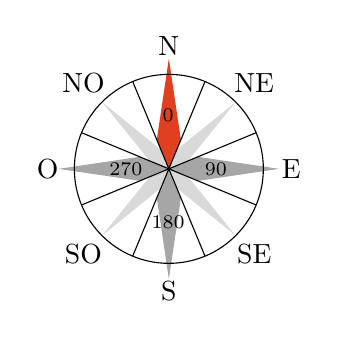
\begin{tikzpicture}[scale=0.4]
    \def\distCardeais{4.5cm}
    \def\distCardeaisValue{2.2cm}
    \def\distColaterais{4.7cm}

    %rosa dos ventos
    \foreach \ang in {0, 180, 270} {
        \fill[gray!70]
            (\ang:3.5cm) -- (\ang+22.5:1.0cm) -- (0,0) -- (\ang-22.5:1.0cm) -- cycle;
%        \fill[gray!50]
%            (\ang:0cm) -- (\ang+10:0.1cm) -- (\ang:0.5cm) -- (\ang-10:0.1cm) -- cycle;
    }
    \foreach \ang in {90} {
        \fill[red!50!brown]
            (\ang:3.5cm) -- (\ang+22.5:1.0cm) -- (0,0) -- (\ang-22.5:1.0cm) -- cycle;
%        \fill[gray!50]
%            (\ang:0cm) -- (\ang+10:0.1cm) -- (\ang:0.5cm) -- (\ang-10:0.1cm) -- cycle;
    }
    \foreach \ang in {45, 135, 225, 315} {
        \fill[gray!30]
            (\ang:3.0cm) -- (\ang+22.5:0.66cm) -- (0,0) -- (\ang-22.5:0.66cm) -- cycle;
    }

    \draw[thin] (0,0) circle(3cm);

    \foreach \ang in {22.5, 67.5, 112.5, 157.5, 202.5, 247.5, 292.5, 337.5} {
        \draw[thin] (0,0) -- (\ang+90:3cm);
    }

    \foreach \ang/\label/\value in {
        90/N/0, 0/E/90, 270/S/180, 180/O/270
    } {
        \node[anchor=\ang] at (\ang:\distCardeais) {\label};
        \node[anchor=\ang] at (\ang:\distCardeaisValue) {$_{\value}$};
    }

    \foreach \ang/\label in {
        135/NO, 225/SO, 315/SE, 45/NE
    } {
        \node[anchor=\ang] at (\ang:\distColaterais) {\label};
    }
\end{tikzpicture}
\end{center}

Implemente o código:
\begin{minted}{custompython}
def bussola(deg: float) -> str:
    # seu código aqui

#teste
print(bussola(20.7))
print(bussola(169.2))
print(bussola(-60.3))
print(bussola(868.5))
\end{minted}

Saída esperada:
\begin{minted}{text}
Norte
Sul
Noroeste
Sudoeste
\end{minted}
